\documentclass[conference,10pt]{IEEEtran}
\usepackage[utf8]{inputenc}
\usepackage[T1]{fontenc}
\usepackage{microtype}
\usepackage{booktabs}
\usepackage{graphicx}
\usepackage{xcolor}
\usepackage{tikz}
\usepackage{amsmath}
\usepackage{balance}
\usetikzlibrary{positioning,arrows.meta,shapes.geometric,calc,fit,backgrounds}
\usepackage[hidelinks]{hyperref}
\usepackage{etoolbox}
% The class puts an em dash after "Abstract" and "Index Terms"; use a colon instead.
\makeatletter
\patchcmd{\abstract}{---}{:\ }{}{\typeout{abstract dash not patched}}
\patchcmd{\IEEEkeywords}{---}{:\ }{}{\typeout{keywords dash not patched}}
\makeatother
\usepackage{caption}
\captionsetup{font=small,labelfont=bf,skip=5pt}

\definecolor{cExr}{HTML}{2D4A6B}
\definecolor{cJson}{HTML}{5B8FB0}
\definecolor{cExrShort}{HTML}{7A9A5A}
\definecolor{cTagged}{HTML}{D99A2B}
\definecolor{cDsl}{HTML}{C4513B}
\definecolor{cWords}{HTML}{8E5A9E}
\definecolor{cCorrect}{HTML}{CFD8CF}
\definecolor{cSilent}{HTML}{C4513B}
\definecolor{cDetectable}{HTML}{E8C48A}
\definecolor{cInk}{HTML}{22303F}
\definecolor{cMuted}{HTML}{8A94A0}
\definecolor{cRule}{HTML}{D7DCE2}

\newcommand{\dslEm}{0.755}
\newcommand{\dslEmSmall}{0.556}
\newcommand{\dslHall}{0.109}
\newcommand{\dslLat}{346}
\newcommand{\dslMiss}{0.233}
\newcommand{\dslSilent}{0.139}
\newcommand{\dslTok}{12.5}
\newcommand{\dslValid}{0.894}
\newcommand{\exrEm}{0.833}
\newcommand{\exrEmSmall}{0.757}
\newcommand{\exrHall}{0.158}
\newcommand{\exrLat}{1213}
\newcommand{\exrMiss}{0.257}
\newcommand{\exrShortEm}{0.591}
\newcommand{\exrShortEmSmall}{0.507}
\newcommand{\exrShortHall}{0.169}
\newcommand{\exrShortLat}{927}
\newcommand{\exrShortMiss}{0.242}
\newcommand{\exrShortSilent}{0.174}
\newcommand{\exrShortTok}{34.0}
\newcommand{\exrShortValid}{0.764}
\newcommand{\exrSilent}{0.163}
\newcommand{\exrTok}{45.4}
\newcommand{\exrValid}{0.996}
\newcommand{\hallRatio}{4.4}
\newcommand{\jsonEm}{0.759}
\newcommand{\jsonEmSmall}{0.694}
\newcommand{\jsonHall}{0.145}
\newcommand{\jsonLat}{1222}
\newcommand{\jsonMiss}{0.210}
\newcommand{\jsonSilent}{0.146}
\newcommand{\jsonTok}{44.5}
\newcommand{\jsonValid}{0.904}
\newcommand{\memMax}{1966}
\newcommand{\memMin}{1705}
\newcommand{\nPcfg}{434}
\newcommand{\nRuns}{36}
\newcommand{\nTest}{1357}
\newcommand{\noiseFloor}{0.043}
\newcommand{\pcfgExr}{0.643}
\newcommand{\pcfgWords}{0.721}
\newcommand{\silentRatio}{2.3}
\newcommand{\speedup}{3.8}
\newcommand{\taggedEm}{0.807}
\newcommand{\taggedEmSmall}{0.758}
\newcommand{\taggedHall}{0.132}
\newcommand{\taggedLat}{651}
\newcommand{\taggedMiss}{0.226}
\newcommand{\taggedSilent}{0.140}
\newcommand{\taggedTok}{22.7}
\newcommand{\taggedValid}{0.947}
\newcommand{\tokRatio}{3.8}
\newcommand{\wordsEm}{0.830}
\newcommand{\wordsEmSmall}{0.727}
\newcommand{\wordsHall}{0.036}
\newcommand{\wordsLat}{322}
\newcommand{\wordsMiss}{0.074}
\newcommand{\wordsSilent}{0.070}
\newcommand{\wordsTok}{11.9}
\newcommand{\wordsValid}{0.900}


% --- on-device numbers -------------------------------------------------------
% MEASURED on an iPad (A16) running iOS 26.3.1 by the client's own benchmark:
% ten representative orders, three timed rounds after a discarded warm-up pass,
% through the same OrderParser the booth uses. Regenerate with the Бенчмарк
% button in the Orders toolbar (triple-tap the wordmark to reveal it); its
% Копировать button emits exactly these macros.
\newcommand{\padDevice}{iPad15,7}
\newcommand{\padLatency}{167\,ms}
\newcommand{\padPninety}{354\,ms}
\newcommand{\padLoad}{2.5\,s}
\newcommand{\padMem}{350\,MiB}
\newcommand{\padTps}{16\,tok/s}
\newcommand{\estnote}{}
% ----------------------------------------------------------------------------

\newcommand{\fmt}[1]{\textsc{#1}}
\newcommand{\code}[1]{{\small\texttt{#1}}}

\tikzset{
  stage/.style={draw=cRule,line width=0.6pt,rounded corners=2pt,fill=white,
                inner sep=4pt,font=\scriptsize,align=center,minimum height=7mm},
  tok/.style={font=\scriptsize\bfseries,inner sep=1pt},
  flow/.style={-{Stealth[length=3pt,width=3pt]},draw=cMuted,line width=0.6pt},
}

\begin{document}

\title{Fewer Tokens, Fewer Silent Errors:\\
Output Format Design for Small Language Models\\
in Real Time Order Parsing}

\author{
\IEEEauthorblockN{Umar Ahmed}
\IEEEauthorblockA{\textit{Independent Researcher}\\
uakhmed@itmo.ru}
\and
\IEEEauthorblockN{Maxim Duanev}
\IEEEauthorblockA{\textit{Independent Researcher}\\
mduanev@itmo.ru}
}

\maketitle

\begin{abstract}
Small language models are cheap to fine tune and fast to serve, but they
hallucinate, and a hallucination that parses cleanly is invisible to the system
that consumes it. We ask whether the \emph{output format} can be designed to
reduce that risk on a narrow task. We fine tune Qwen3.5-0.8B with LoRA on the
public PIZZA semantic parsing benchmark using six lossless encodings of the same
target tree, arranged as a ladder from \exrTok{} down to \wordsTok{} tokens per
utterance, with two matched token pairs that hold length fixed while varying
surface form. Across \nRuns{} runs we find that shortening the output does
\emph{not} by itself improve accuracy: at 1000 training examples every ten tokens
removed costs about four points of exact match. What matters is whether the
surface form is made of natural words. A word based encoding matches the native
s-expression on accuracy (\wordsEm{} versus \exrEm{}, inside a measured rerun
noise floor of \noiseFloor{}) while using \tokRatio{}$\times$ fewer tokens,
running \speedup{}$\times$ faster at batch size one, producing
\hallRatio{}$\times$ fewer hallucinated entities, and halving the rate of errors
that parse cleanly but are wrong. We argue this last quantity, which we call the
\emph{silent error rate}, is the right objective for deploying small models, and
we report a café ordering system that runs at 80\,ms per order on a consumer
laptop.
\end{abstract}

\begin{IEEEkeywords}
semantic parsing, small language models, hallucination, LoRA, output formats
\end{IEEEkeywords}

\section{Introduction}

A small language model is attractive for a narrow task. It fine tunes in minutes,
runs on a laptop, and costs almost nothing per call. The objection is
reliability: small models hallucinate, and in a structured output setting a
hallucination is not an obviously broken string. It is a well formed tree
describing an order nobody placed.

This distinction matters more than overall accuracy. An output that fails to
parse is a \emph{detectable} failure: the caller sees it, rejects it, and retries.
An output that parses but is wrong is a \emph{silent} failure: the caller has no
signal, and a customer receives the wrong order. We therefore separate the two
and treat the silent rate as the quantity to minimise.

Our question is whether the target format itself is a lever. The same semantic
tree can be written many ways, and the choice changes how many tokens the model
must emit, how fast it responds, and apparently how often it invents content.
Our initial hypothesis was simple: fewer output tokens should mean less room to
hallucinate, faster responses, and cheaper fine tuning.

That hypothesis is not supported in the form we posed it. Shortening the output
alone does not improve accuracy, and at low data it clearly hurts. But a sharper
version survives: shortening helps when the surface form stays close to natural
language, and hurts when it becomes symbolic. Section~\ref{sec:results} shows
this with matched token controls that separate length from form.

\textbf{Contributions.}
(1) A ladder of six lossless encodings of the PIZZA target tree spanning
\exrTok{} to \wordsTok{} tokens, with matched token pairs that isolate length
from surface form.
(2) Evidence that length alone is not the mechanism, from twelve paired
comparisons that all separate.
(3) The silent error rate as a deployment objective, with a word based encoding
halving it relative to the native format.
(4) A measured rerun noise floor of \noiseFloor{} exact match, which bounds
what any three seed comparison on this task can claim.

\begin{figure}[t]
\centering
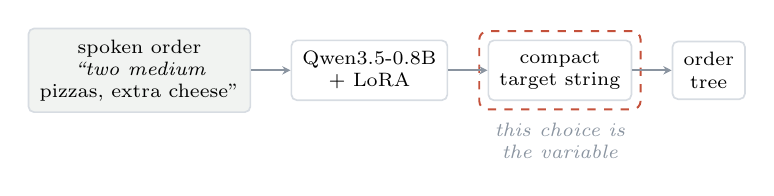
\begin{tikzpicture}
  \node[stage,fill=cCorrect!30] (a) {spoken order\\\scriptsize\itshape ``two medium\\pizzas, extra cheese''};
  \node[stage,right=5mm of a] (b) {Qwen3.5-0.8B\\+ LoRA};
  \node[stage,right=5mm of b] (c) {compact\\target string};
  \node[stage,right=5mm of c] (d) {order\\tree};
  \draw[flow] (a) -- (b);
  \draw[flow] (b) -- (c);
  \draw[flow] (c) -- (d);
  \node[below=1.5mm of c,font=\scriptsize\itshape,text=cMuted,align=center]
    {this choice is\\the variable};
  \begin{scope}[on background layer]
    \node[draw=cSilent,line width=0.7pt,rounded corners=3pt,dashed,
          fit=(c),inner sep=3pt] {};
  \end{scope}
\end{tikzpicture}
\caption{The pipeline. Everything is held fixed except the format the model is
trained to emit.}
\label{fig:pipeline}
\end{figure}

\section{Task and System}

\subsection{The café parser}
\label{sec:coffee}

The work began with a deployed system. A café ordering booth must turn a spoken
order, already transcribed, into a structured ticket. Orders arrive in Russian
and English, with diminutives, self corrections and off menu items. We fine tuned
Qwen3.5-0.8B with LoRA on a synthetic generator covering ten drinks, three sizes,
five milks and three syrups, with a compact target format:

\begin{center}
\code{cap L oat;lat x2}
\end{center}

where each item is \code{drink [size] [milk] [syrup] [xN]} and \code{?} marks an
utterance that is not an order. On a hand written 49 case evaluation set, written
separately from the generator and containing slang the generator never produces,
the model reaches 48 of 49, emitting about three output tokens per order with a
median latency of 80\,ms. That figure is measured on an Apple M1 through a
local Ollama server using the same Q8\_0 GGUF, which is 795\,MiB on disk. The
compact format uses roughly three times fewer output tokens than an equivalent
JSON encoding, which is most of that latency.

This system works, but it cannot support a claim. The evaluation set is small,
and the same author wrote both the generator and the test cases. To say anything
general we moved to a public benchmark.

\subsection{PIZZA}

PIZZA~\cite{pizza} is a semantic parsing dataset of spoken pizza and drink
orders paired with executable target trees. We use the public 10\% training pool
of 245{,}645 utterances, the 348 utterance development split and the \nTest{}
utterance test split, of which \nPcfg{} are marked as failures of the authors'
PCFG baseline. Targets look like:

\begin{center}
\footnotesize\ttfamily
(ORDER (PIZZAORDER (NUMBER 2 )\\
(SIZE MEDIUM ) (COMPLEX\_TOPPING\\
(QUANTITY EXTRA ) (TOPPING CHEESE ) ) ) )
\end{center}

We verified that no development or test utterance appears in the training pool,
exactly or after normalisation, at any training size or seed.

\section{Output Format Ladder}

Comparing unrelated formats confounds length with surface form. We instead built
six encodings of the \emph{identical} tree that round trip to byte identical
targets, four forming a length ladder and two held at matched length.

\begin{figure}[t]
\centering
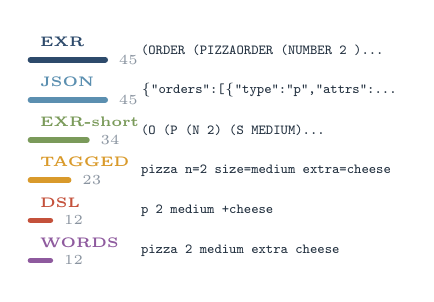
\begin{tikzpicture}[node distance=0pt]
  \def\rowsep{5.1mm}
  \foreach \i/\name/\col/\tok/\txt in {
    0/EXR/cExr/45/{(ORDER (PIZZAORDER (NUMBER 2 )...},
    1/JSON/cJson/45/{\{"orders":[\{"type":"p","attrs":...},
    2/EXR-short/cExrShort/34/{(O (P (N 2) (S MEDIUM)...},
    3/TAGGED/cTagged/23/{pizza n=2 size=medium extra=cheese},
    4/DSL/cDsl/12/{p 2 medium +cheese},
    5/WORDS/cWords/12/{pizza 2 medium extra cheese}}
  {
    \node[anchor=west,font=\tiny\bfseries,text=\col]
      at (0,-\i*\rowsep) {\name};
    \draw[\col,line width=2pt,line cap=round]
      (0,-\i*\rowsep-2.3mm) -- ++({\tok/45*0.95},0);
    \node[anchor=west,font=\tiny,text=cMuted]
      at ({\tok/45*0.95+0.05},-\i*\rowsep-2.3mm) {\tok};
    \node[anchor=west,font=\tiny\ttfamily,text=cInk]
      at (1.28,-\i*\rowsep-1.1mm) {\txt};
  }
\end{tikzpicture}
\caption{The six encodings, all lossless and all preserving the dataset's own
sibling order. \fmt{EXR}/\fmt{JSON} and \fmt{DSL}/\fmt{WORDS} are matched token
pairs: nearly equal length, different surface form.}
\label{fig:ladder}
\end{figure}

\fmt{EXR} is the dataset's native s-expression. \fmt{JSON} is a conventional
structured encoding at nearly identical token count. \fmt{EXR-short} replaces
constructor names with single letters. \fmt{TAGGED} is flat \code{key=value}
pairs. \fmt{DSL} is a compact grammar with sigils, where \code{+} marks an extra
quantity and \code{!} a negation. \fmt{WORDS} shares the DSL's structure but
spells markers out as ordinary words.

All six decode back to the identical tree on every development and test
utterance and on a 50{,}000 example training sample, checked against the
dataset's own matcher.

\paragraph{A tokenizer floor.}
We also built a seventh encoding using short opaque entity codes, for example
\code{p !p5 2 m3 +c2}. It has 16.4 characters per utterance against the DSL's
34.9, less than half, but \emph{more} tokens, 11.9 against 10.8, because codes
outside the subword vocabulary fragment. Shortening the string stops reducing
tokens well before the information content does. This is why no arm sits below
roughly ten tokens.

\section{Experimental Setup}

Identical across all arms: Qwen3.5-0.8B, LoRA with $r{=}16$, $\alpha{=}16$ on all
attention and MLP projections, batch 16, cosine schedule, loss on the completion
only. The prompt is the same template the café model uses. Learning rate is
selected per arm from $\{1\mathrm{e}{-4}, 2\mathrm{e}{-4}, 5\mathrm{e}{-4}\}$ on
development exact match at $n{=}20{,}000$ across three seeds, then frozen.
Training uses early stopping on development exact match with patience 10,
evaluated every 100 steps, to a maximum of 4000 steps.

\texttt{max\_new\_tokens} is set per arm to the longest target across all splits
times 1.25, so no gold length output can be truncated. We log the share of
generations reaching that cap; it is zero for every reported run.

Development drives every decision. Test is evaluated once per run and never read
by any selection step. Exact match always comes from the dataset's own unordered
matcher, which we never reimplement.

\paragraph{Noise floor.}
We retrained one configuration twice under identical settings. Test exact match
differed by \noiseFloor{}. Any difference smaller than this is indistinguishable
from rerun variance, and we do not interpret such differences.

\section{Results}
\label{sec:results}

\begin{table*}[t]
\centering
\caption{Test results at $n{=}20{,}000$, mean of three seeds. Silent error is
the share of utterances that parse cleanly but do not match the gold tree: the
caller cannot detect these. Latency is median at batch size one on a shared GPU,
and memory is this process's own GPU allocation during that measurement.}
\label{tab:main}
\small
\begin{tabular}{lrrrrrrr}
\toprule
Format & Tokens & Exact match & Parse validity & \textbf{Silent error} & Halluc./utt.\ & Latency (ms) & Mem.\ (MiB) \\
\midrule
EXR & 45.4 & 0.833 {\scriptsize $\pm$ 0.015} & 0.996 & 0.163 & 0.158 & 1213 & 1966 \\
JSON & 44.5 & 0.759 {\scriptsize $\pm$ 0.017} & 0.904 & 0.146 & 0.145 & 1222 & 1707 \\
EXR-short & 34.0 & 0.591 {\scriptsize $\pm$ 0.061} & 0.764 & 0.174 & 0.169 & 927 & 1706 \\
TAGGED & 22.7 & 0.807 {\scriptsize $\pm$ 0.037} & 0.947 & 0.140 & 0.132 & 651 & 1706 \\
DSL & 12.5 & 0.755 {\scriptsize $\pm$ 0.042} & 0.894 & 0.139 & 0.109 & 346 & 1705 \\
WORDS & 11.9 & 0.830 {\scriptsize $\pm$ 0.031} & 0.900 & 0.070 & 0.036 & 322 & 1705 \\
\bottomrule
\end{tabular}

\end{table*}

\begin{figure}[t]
\centering
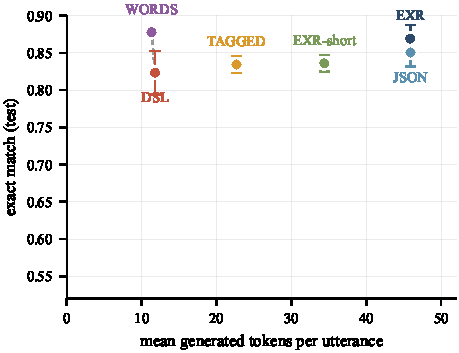
\includegraphics[width=\columnwidth]{figures/accuracy_vs_tokens}
\caption{Accuracy against output length. Dashed lines join the matched token
pairs: within each pair length is held nearly constant, yet accuracy differs.
Length alone does not determine accuracy.}
\label{fig:acc}
\end{figure}

\subsection{Shorter is not automatically better}

Table~\ref{tab:main} and Figure~\ref{fig:acc} show no monotone benefit from
shortening. Regressing exact match on mean generated tokens across the four
ladder arms gives a \emph{positive} slope at both training sizes: at $n{=}1000$,
removing ten tokens costs about four points of exact match. \fmt{EXR-short}, the
most aggressive structural compression, is the worst arm at \exrShortEm{}, with
parse validity of only \exrShortValid{}. Our original hypothesis, stated as
``fewer output tokens is better,'' is falsified.

\subsection{Surface form, not length}

The matched token pairs separate the two explanations, and all twelve
comparisons separate under a paired bootstrap over the \nTest{} test utterances.

\begin{table}[t]
\centering
\caption{Matched token pairs at $n{=}20{,}000$. Paired bootstrap over test
utterances. Equal length, different surface form, consistently different
accuracy.}
\label{tab:matched}
\scriptsize
\setlength{\tabcolsep}{3.5pt}
\begin{tabular}{llrrrl}
\toprule
Pair & Seed & Tokens & $\Delta$ EM & 95\% CI & Verdict \\
\midrule
EXR/JSON & 0 & 45.3/44.9 & +0.069 & [+0.046,\,+0.091] & sep. \\
EXR/JSON & 1 & 45.3/44.8 & +0.088 & [+0.069,\,+0.108] & sep. \\
EXR/JSON & 2 & 45.6/43.7 & +0.066 & [+0.043,\,+0.090] & sep. \\
DSL/WORDS & 0 & 12.5/12.1 & -0.077 & [-0.099,\,-0.057] & sep. \\
DSL/WORDS & 1 & 12.5/11.7 & -0.046 & [-0.069,\,-0.023] & sep. \\
DSL/WORDS & 2 & 12.4/12.0 & -0.101 & [-0.127,\,-0.074] & sep. \\
\bottomrule
\end{tabular}

\end{table}

\fmt{DSL} and \fmt{WORDS} differ by less than a token in length, yet \fmt{WORDS}
wins every seed. The two encode the same structure; they differ only in whether
a quantity marker is written \code{+cheese} or \code{extra cheese}. Symbolic
surface forms cost accuracy that natural word forms do not.

\subsection{Silent errors}

\begin{figure}[t]
\centering
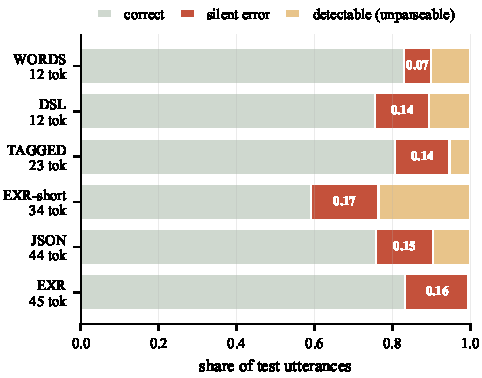
\includegraphics[width=\columnwidth]{figures/error_composition}
\caption{Where the test set goes for each format, ordered by output length.
Silent errors parse cleanly but are wrong, so a downstream system cannot detect
them. Detectable failures can be rejected and retried.}
\label{fig:errors}
\end{figure}

Figure~\ref{fig:errors} is the deployment picture. \fmt{EXR} has the highest
parse validity at \exrValid{}, but that is not an unalloyed good: nearly
everything it gets wrong, it gets wrong \emph{silently}, at \exrSilent{}.
\fmt{WORDS} parses less often, \wordsValid{}, but its silent rate is
\wordsSilent{}, a factor of \silentRatio{} lower. Its errors surface as parse
failures a caller can catch.

The hallucination counts move the same way: \wordsHall{} invented entities per
utterance against \exrHall{} for \fmt{EXR}, a factor of \hallRatio{}, and
\wordsMiss{} missing entities against \exrMiss{}.

\subsection{Latency}

\begin{figure}[t]
\centering
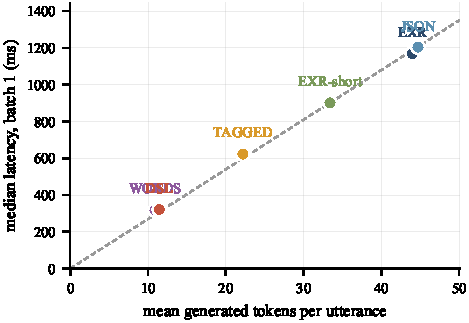
\includegraphics[width=\columnwidth]{figures/latency_vs_tokens}
\caption{Median latency at batch size one is close to linear in generated
tokens. Throughput in tokens per second is flat across formats, so the speedup
comes from emitting less, not from running faster.}
\label{fig:latency}
\end{figure}

Latency is close to proportional to output length
(Figure~\ref{fig:latency}). \fmt{WORDS} responds in \wordsLat{}\,ms against
\exrLat{}\,ms for \fmt{EXR}, a \speedup{}$\times$ speedup, on a shared GPU under
contention from other tenants. Tokens per second is flat across arms, confirming
the gain comes from length rather than from a faster model.

Memory tells a different story. Across all eighteen measurements the process
holds between \memMin{} and \memMax{}\,MiB, a spread of about fifteen percent
that tracks the longer key value cache the verbose formats need. Weights
dominate, and those are identical across arms. \textbf{Format choice buys
latency and accuracy, not memory.} A practitioner picking a format to fit a
memory budget is picking the wrong lever; the lever for memory is quantisation,
which is what the deployed client in Section~\ref{sec:ipad} uses.

\subsection{Data efficiency}

\begin{figure}[t]
\centering
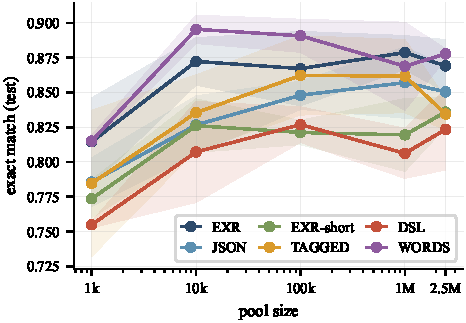
\includegraphics[width=\columnwidth]{figures/data_efficiency}
\caption{Exact match against training set size. The penalty for symbolic formats
is largest when data is scarce, and narrows as data grows.}
\label{fig:data}
\end{figure}

Figure~\ref{fig:data} shows the format penalty is a low data phenomenon. At
$n{=}1000$, \fmt{DSL} reaches \dslEmSmall{} against \fmt{WORDS} at
\wordsEmSmall{}. By $n{=}20{,}000$ the gap narrows. A format closer to natural
language appears to let the model reuse what pretraining already gave it, which
matters most when there is little task data to learn from.

\subsection{Deployment on device}
\label{sec:ipad}

The café parser runs entirely on an iPad, with no network call. The client is a
SwiftUI application that links llama.cpp as an \texttt{xcframework} and offloads
every layer to the Metal GPU. Table~\ref{tab:device} lists what it costs to
carry.

\begin{table}[h]
\centering
\caption{On-device footprint, measured on an iPad (A16) by the client's own
benchmark: ten representative orders, three timed rounds after a discarded
warm-up pass. The model is the café parser quantised to Q8\_0.\estnote}
\label{tab:device}
\footnotesize
\setlength{\tabcolsep}{4pt}
\begin{tabular}{ll}
\toprule
Device & \padDevice, iOS 26.3 \\
Base model & Qwen3.5, 0.773\,B parameters, 25 blocks \\
Quantisation & Q8\_0, 8.63 bits per weight \\
Model file & 795\,MiB \\
Inference runtime & llama.cpp, 11\,MiB framework (arm64) \\
GPU offload & all layers, Metal \\
Context window & 512 tokens \\
Peak resident footprint & \padMem \\
Model load time & \padLoad \\
Median latency & \padLatency \\
p90 latency & \padPninety \\
Throughput & \padTps \\
\bottomrule
\end{tabular}
\end{table}

The spread between the median and the p90 is itself the paper's argument,
restated on the hardware a customer waits in front of. Across the ten orders the
benchmark parses, latency is close to linear in the number of output tokens:
a least squares fit gives 48\,ms of fixed overhead plus 52\,ms per generated
token ($R^2 = 0.91$), so a one token reply such as \code{esp} returns in about
100\,ms while the longest, a seven token two drink order, takes about 414\,ms.
The format's token count is therefore not a throughput abstraction but the
dominant term in the wait, and the \tokRatio{}$\times$ reduction the word based
encoding buys becomes the same factor of responsiveness at the booth.

The footprint deserves a note, because \padMem{} is well under the 795\,MiB
model file. The figure is \texttt{phys\_footprint}, which is what iOS enforces
its per-process memory limit against, and llama.cpp maps the weight file rather
than copying it, so the weight pages are file backed and are reclaimable under
pressure instead of counting against that limit. The number to plan a deployment
around is therefore the resident figure, not the file size, and on this device it
leaves the parser a long way inside the budget of even an entry level iPad.

Two further details matter for reproducibility. First, the prompt template and
the three stop strings compiled into the client are byte identical to those used
for training and for every evaluation in this paper, so the deployed model sees
exactly the input distribution it was fitted on. Second, the context window is
512 tokens, which the compact format fits comfortably and the equivalent JSON
encoding would not at the longest orders. A format chosen for token count at
training time therefore also decides whether the model fits a small on-device
context at serving time.

The practical consequence is that a booth needs no server, no network round
trip, and no per-request cost. The whole parser is a 795\,MiB file beside an
11\,MiB runtime.

\subsection{Reproducibility}

Every number in this paper is recomputed from saved model outputs rather than
copied from a training log. Each of the \nRuns{} runs writes its configuration,
package versions, training curves, adapter weights and the full prediction file
for both evaluation splits. A prediction row carries the source utterance, the
gold tree, the raw model output, the parsed tree or a null, a correctness flag
and the generated token count, so exact match can be recomputed offline with no
GPU. Every table and figure here is produced by two scripts that read only those
files. The protocol, including the stopping rules and the statements this work
declines to make, was written before any run and records its own later
amendments.

\section{Discussion}

\paragraph{Which format should a practitioner choose?}
\fmt{WORDS}. It ties the native format on accuracy within the noise floor, and
wins on every deployment axis: \tokRatio{}$\times$ fewer tokens,
\speedup{}$\times$ lower latency, \hallRatio{}$\times$ fewer hallucinations, and
\silentRatio{}$\times$ fewer silent errors. The recipe is to compress the
\emph{structure} while keeping the \emph{vocabulary} natural.

\paragraph{Can a small model do this at all?}
At 20{,}000 training examples a 0.8B model reaches \exrEm{} exact match. The
published BART-Large result on this benchmark is 0.786, but it used 2.46M
training examples, 123 times more. We do not claim to beat it. The useful
statement is that comparable accuracy is reachable at a small fraction of the
data and at a model size that serves in real time on consumer hardware, which
the café system in Section~\ref{sec:coffee} does at 80\,ms per order.

\paragraph{Limitations.}
One task, one model, one tokenizer. The tokenizer floor is specific to this
subword vocabulary. Three seeds per cell gives wide intervals, which is why
arm comparisons use a paired bootstrap over utterances rather than seed means.
Learning rate is tuned at $n{=}20{,}000$ and reused at $n{=}1000$. Latency is
measured on a contended shared GPU, so absolute milliseconds are inflated,
though every arm meets the same contention. We have not tested whether these
findings transfer to a larger model, where the format penalty may vanish.

\section{Conclusion}

Output format is a free design variable that changes hallucination rate and
latency by factors of three to four. The intuition that fewer tokens is safer is
not quite right. What helps is compressing structure while keeping the surface
in natural words, and what matters for deployment is not overall accuracy but
how often a model is wrong in a way nobody can detect.

\balance
\begin{thebibliography}{9}
\bibitem{pizza}
K.~Arkoudas \emph{et al.}, ``PIZZA: A new benchmark for complex end-to-end
task-oriented parsing,'' 2022. Dataset:
\url{https://github.com/amazon-science/pizza-semantic-parsing-dataset}
\end{thebibliography}

\end{document}
